\documentclass[12pt]{article}
\usepackage[utf8]{inputenc}
\usepackage{amsmath,amssymb}
\usepackage{unicode-math}
\usepackage[T2A]{fontenc}
\usepackage[russian]{babel}
\usepackage{graphicx}
\usepackage{subfigure}
\usepackage{subcaption}
\usepackage{url}
\usepackage{float}


\DeclareGraphicsExtensions{.pdf,.png,.jpg}
\usepackage{hyperref}
\usepackage{wrapfig}
\usepackage[left=20mm, top=20mm, right=10mm, bottom=20mm]{geometry}

\usepackage{amsmath} 
\usepackage{amsfonts} 
\usepackage{amssymb} 
\usepackage{wasysym} 
\usepackage{fancyhdr}

\pagestyle{fancy}
\fancyhf{}
\lhead{Семинар 10. Ядерные реакции}
\rhead{\textit{Клименок К.Л., МФТИ 2020}}
\rfoot{\thepage}



\begin{document} 
\title{\textbf{Семинар 10. Ядерные реакции }}
\author{\textbf{Клименок Кирилл Леонидович}}
\date{18.11.2020}
\maketitle
\section{Теоретическая часть}
Мы уже поговорили про распады, но, к сожалению или к счастью, этим ядерный мир не ограничивается и сегодня мы посмотрим на то, что происходит, когда ядра разного состава могут взаимодействовать между собой.
\subsection{Сечение реакции}
Начнем с очень простой модели, которую мы уже рассматривали в рамках термодинамики во втором семестре, а именно простое столкновение шариков между собой. Как же это связанно с ядреными реакциями? Самым прямым образом --- чтобы ядерная реакция произошла 2 ядра должны как минимум столкнуться вот для этого мы и можем ввести сечение. Смысл сечения как раз и показывает вероятность той или иной реакции пройти, а размерность совпадает с размерностью площади.
\begin{figure}[h]
    \centering
    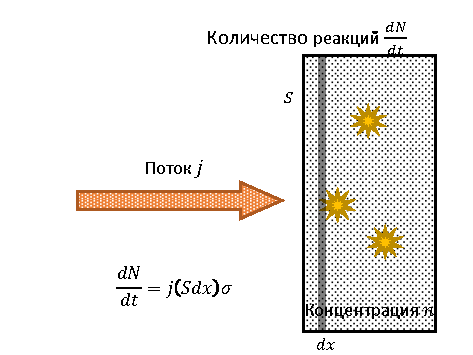
\includegraphics[width=0.5\textwidth,height=\textheight,keepaspectratio]{Seminar_10/pics/pic_01_sigma.pdf}
    \caption{Схема для вывода сечения реакции через налетающий поток частиц}
    \label{fig:sem_10_sigma}
\end{figure}
Теперь опять добавим щепотку математики для картинки выше. Пусть у нас есть поток налетающих частиц $j$ и мишень с концентрацией ядер $n$. Посмотрим сколько реакций за единицу времени $dN/dt$ будет происходить. Очевидно, что скорость будет пропорциональна налетающему потоку и количеству ядер в слое, где мы рассматриваем реакции $nSdx$, но тогда, чтобы соблюсти размерность нам как раз и надо домножить на что-то с размерностью площади, это и будет сечение. То есть:
\begin{equation*}
    \dfrac{dN}{dt} = j (nSdx) \sigma
\end{equation*}
Естественно, измерять сечения в квадратных метрах в микромире неудобно и вводят единицу барн, которая равна $10^{-24}$ $\text{см}^2$.

\begin{figure}[h]
    \centering
    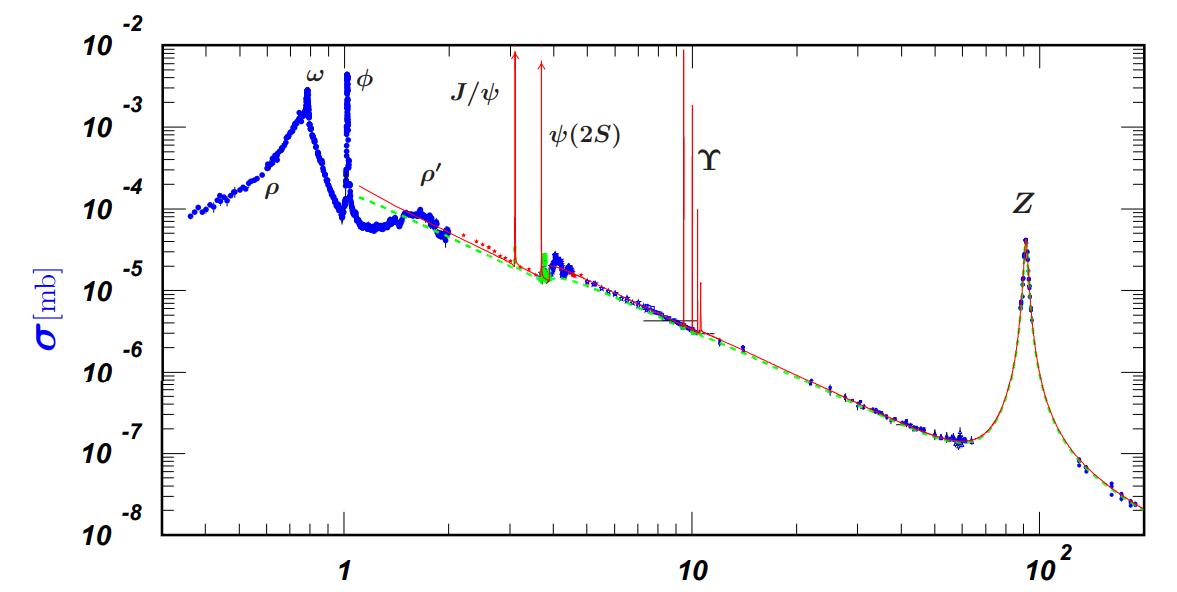
\includegraphics[width=0.9\textwidth,height=\textheight,keepaspectratio]{Seminar_10/pics/pic_02_barn.PNG}
    \caption{Зависимость сечения реакции от энергии налетающих частиц}
    \label{fig:sem_10_barn}
\end{figure}

Теперь давайте посмотрим на характерную картиночку для зависимости сечения реакции от энергии налетающих частиц то мы увидим 2 особенности:
\begin{itemize}
    \item Наличие около линейного спада во всех диапазонах энергий
    \item Какие-то очень похожие на резонанс пики
\end{itemize}
Вот именно их мы и попытаемся описать в рамках наших моделей

\subsection{Нерезонансные реакции. Закон Бете}
Как обычно, нам нужно собрать какую-то модельку, которая бы как-то описывала что вообще происходит с ядром при реакции. Идея очень напоминает идею переходного комплекса в химии, а если говорить по простому то это идея составного ядра. Суть ее в том, что налетающее ядро или частица попадает внутрь ядра, образуется большая нестабильная структура, которая в дальнейшем может распасться на что-то. И то на что распадается это составное ядро называется каналом реакции:
\begin{equation*}
    a + A \rightarrow P^* \rightarrow 
    \begin{cases}
         A + a \text{ <<упругий канал>>}\\
         B + b \text{ другие каналы}\\
         C + c \text{ другие каналы}
    \end{cases}
\end{equation*}
Теперь давайте посмотрим что происходит с частицей которая влетает в ядро. Из-за того что ядро это потенциальная яма с глубиной порядка $U_0 \sim 100$ МэВ, а налетающая частица представляет из себя волну де Бройля, то это должно вам напомнить задачу о пролете частицы над ямой из семинаров 4-5, ведь для нее есть возможность и отразиться от ямы. Тогда окончательно мы можем записать сечение как произведение вероятности <<попасть>> в ядро и вероятности пройти через него:
\begin{gather*}
    \sigma \approx 4\pi (\lambda + R)^2 D(E) = 4\pi (\lambda + R)^2 \dfrac{4k\kappa}{(k+\kappa)^2} \approx 16\pi (\lambda + R)^2 \sqrt{\dfrac{E}{U_0}}\\
    \lambda \sim \dfrac{1}{p} \sim \dfrac{1}{\sqrt{E}}\\
    \sigma \sim \dfrac{\sqrt{E}}{E} \sim \dfrac{1}{\sqrt{E}} \sim \dfrac{1}{v}
\end{gather*}
Здесь как и раньше $k = \sqrt{\dfrac{2mE}{\hbar^2}}$ и $ \kappa = \sqrt{\dfrac{2m(U_0 + E)}{\hbar^2}}$, $v$ --- скорость налетающей частицы. Как нам это интерпретировать? Все максимально просто и имеет классическую аналогию с пулей и мишенью. Если скорость пули маленькая, то она застревает в мишени, а если большая --- прошивает ее насквозь и улетает, куда-то дальше. 
\subsection{Резонансные реакции. Формула Брейта-Вигнера}
Так, общий тренд мы уловили, а теперь давайте обсудим, что делать с резонансами. Во-первых, разберемся, почему они физически появляются. Тут все просто, если резонанс есть, это означает, что мы так угадали энергию налетающей частицы, что наше составное ядро может существовать какое-то время само может существовать. почему же тогда у нас могут быть разные по ширине резонансные пики? Тут все еще проще, есть соотношение неопределенностей энергия-время $E\tau \approx \hbar$ и получается, что ширина линии обратно пропорциональна времени жизни. Теперь что же с точки зрения математики? Здесь мы не будем выводить формулу, а просто запишем ее по аналогии со структурой резонансной линии из задачек про колебания:
\begin{gather*}
    \sigma_{ab} = \pi \lambda^2 \dfrac{\Gamma_a \Gamma_b}{(E-E_0)^2 + \Gamma^2/4}\\
    \Gamma = \Gamma_a + \Gamma_b + \dots\\
    \dfrac{\Gamma_a}{\Gamma_b}=\dfrac{\tau_b}{\tau_a}
\end{gather*}
Теперь разбираемся с буквами в этой формуле. Первый множитель с длиной волны нужен нам чтобы совпасть по размерности и идея из закона Бете сохраняется. Разность $E-E_0$ тоже достаточно понятна --- просто положение резонанса на энергии $E_0$ и энергия налетающей частицы $E$. Теперь с буквами $\Gamma$. Они имеют размерность энергии и несут в себе смысл обратных времен составного ядра, а индекс соответствует каналу по которому оно распадается (опять же это берется из соотношения неопределнностей $\Gamma \tau \approx \hbar$) 
\subsection{Ядерные реакторы}
Тут должен был быть разговор про цепные ядерные реакции и то как реактор устроен и управляется, но все задачи из задания по этой теме в задачнике решены. Из основных идей которые надо сказать это написать саму реакцию деления ядра урана:
\begin{equation*}
    n + ^{235}U \rightarrow ^{92}Kr + ^{141}Ba + 3n
\end{equation*}
Мы видим, что при делении появляется больше нейтронов, чем в нее влетает, таким образом можно сказать, что один нейтрон может породить цепную реакцию деления урана. Такая реакция есть и возможна в атомной бомбе и проблема в том, что она неконтролируема. Если же мы посмотрим на вылетевшие нейтроны, то они будут с характерной энергией для ядра порядка МэВ, и их нужно замедлить, чтобы повысить вероятность провзаимодействовать с ядром урана (там нужна энергия нейтронов порядка эВ) для этого можно использовать или тяжелую воду или графит. Время такого торможения составляет микросекунды и на таком масштабе мы не можем регулировать реактор. Но нам везет и механизм поддержания реакции в критическом режиме, когда не происходит ни рост ни уменьшение числа нейтронов, основан на реакции 
\begin{equation*}
    ^{87}Kr \rightarrow ^{86}Kr + n
\end{equation*}
Исходное вещество получается как продукт дальнейших распадов дочерних ядер, а <<запаздывающие>> нейтроны из этой реакции появляются через минуту и именно их количество можно контролировать.

\section{Практическая часть}
\subsection{Задача 8.45}
\label{task_}
\paragraph{Условие}
При просвечивании детали тепловыми нейтронами с длиной волны $\lambda = 1$ \AA на изображении было обнаружено темное пятно, свидетельствующее о наличии инородного включения. Контраст (отношение интенсивности прошедших нейтронов к падающим) был равен 1.26. Какова должна быть длина волны нейтрона, чтобы контраст вырос до 2.
\paragraph{Решение}
\begin{figure}[h]
    \centering
    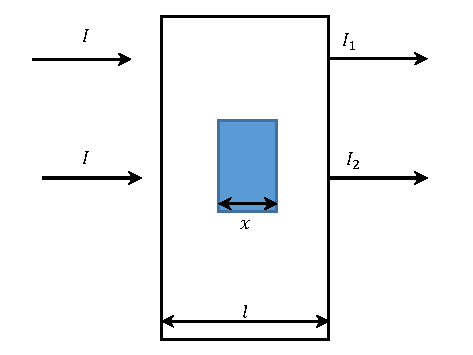
\includegraphics[width=0.4\textwidth,height=\textheight,keepaspectratio]{Seminar_10/pics/pic_03_8_45.pdf}
    \caption{Рисунок к задаче 8.45}
\end{figure}
Эта задачка на нерезонансную реакцию и закон Бете. Мы знаем уравнение на количество реакций в единице толщины и можем его проинтегрировать по всей длине нашего включения:
\begin{equation*}
    \dfrac{dN}{dt} = j (nSdx) \sigma \Rightarrow \dfrac{dN}{Sdt} = \dfrac{dj}{dx}= - j n \sigma \Rightarrow j(x) = j_0 \exp{(-n\sigma x)}
\end{equation*}
Тогда 
\begin{gather*}
    I_1 = I \exp{[-n_1\sigma_1 l]}\\
    I_2 = I \exp{[-n_1\sigma_1 (l-x)-n_2\sigma_2 x]}\\
    \dfrac{I_2}{I_1} = \exp{[x(n_2\sigma_2 - n_1\sigma_1)]} = 1.26
\end{gather*}
Теперь приплетем сюда закон Бете и скажем, что $\sigma \sim 1/v \sim \lambda$ и тогда безнаказанно добавим в показатель экспоненты множитель $q$:
\begin{gather*}
    \dfrac{I'_2}{I'_1} = \exp{[xq(n_2\sigma_2 - n_1\sigma_1)]} = 2
\end{gather*}
Решая это уравнение получаем, что $q = 3$, то есть ответ в 3 раза.

\subsection{Задача 8.68}
\paragraph{Условие}
При облучении ядра $^{115}In$ нейтронами с энергией $E_n = 1.44$ эВ происходит их резонансное поглощение. Распад составного ядра происходит по двум каналам --- радиационному (с испусканием $\gamma$-квантов) и упругому (с вылетом нейтрона). Полное сечение этой реакции равно $\sigma_0 = 2.7 \cdot 10^4$ бн. Ширина нейтронного канала распада $\Gamma_n = 1.2 \cdot 10^{−3}$ эВ. Оценить среднее время жизни составного ядра относительного испускания $\gamma$-квантов,
считая, что $\Gamma_{\gamma} \gg \Gamma_n$. Частицы считать бесспиновыми.
\paragraph{Решение}
Ну тут все должно начинаться с формулы Брейта-Вигнера для резонансного случая $E = E_0$:
\begin{gather*}
    \sigma_{n, \gamma} = 4\pi \lambda^2 \dfrac{\Gamma_n \Gamma_{\gamma}}{(\Gamma_n +\Gamma_{\gamma})^2} \approx 4\pi \lambda^2 \dfrac{\Gamma_n}{\Gamma_{\gamma}} \approx \sigma_0
\end{gather*}
Так как ширины каналов имеют смысл вероятностей процессов то, сечение излучения $\gamma$-кванта будет много больше чем, чем сечение упругого рассеяния и тогда:
\begin{gather*}
    \sigma_{n, \gamma}  \approx \sigma_0 \approx 4\pi \lambda^2 \dfrac{\Gamma_n}{\Gamma_{\gamma}} \Roghtarrow \Gamma_{\gamma} \approx  4\pi \lambda^2 \dfrac{\Gamma_n}{\sigma_0}\\
\end{gather*}

Ну а как у нас время жизни связано с шириной канал мы уже говорили:
чем сечение упругого рассеяния и тогда:
\begin{gather*}
    \tau = \dfrac{\hbar}{\Gamma_{\gamma}} \approx 10^{-15} \text{ с}\\
\end{gather*}




\subsection{Комментарии к задачам из задания}
\paragraph{Нулевки} Первая это задачка по механике, а вторая про формулку из самого начала
\paragraph{Задача 7.10} Тут закон сохранения импульса и закон сохранения энергии, а для нейтрино ее связь энергии и импульса $E_{\nu} = p_{\nu}c$
\paragraph{Задача 8.45} Решена
\paragraph{Задача 8.62} Тут нужно написать кинетическое уравнение того что происходит с аргоном: почему растет и почему уменьшается, а дальше проинтегрировать. 
\paragraph{Задача 8.68} Решена
\paragraph{Задача 9.4} Решена в задачнике
\paragraph{Задача 9.11} Решена в задачнике

\end{document}
